\chapter{Appendix: HP Bypass Hardware Implementation}
\label{appC}


A method has been proposed to achieve below 3 $\mu s$ switch-over of
ports' role and state (as understood in RSTP specification \cite{IEEE8021D}),
and consequently HP Traffic routing. The solution takes advantage of the fact
that HP Traffic is routed using HP Bypass (see
Chapter~\ref{jitterDeterminismNetworkDimention}). Hardware implementation of HP
Bypass and the simplicity of routing, enables extremely fast port switch-over.
The changes proposed thereafter, shall be integrated into HP Bypass
implementation.

Two registers arranged in a table shall be available per port (RSTP Port Role
Table). A table entry is adressed by VLAN ID. Each entry in the table
represents an association between VLAN number and port's role in this particular
VLAN. An entry size shall be 4 bits to enable encoding the following roles:
Root, Designated, Alternate, Backup, Blocked. There shall be $2^10$ entries
in the register to represent 1024 VLANS. One of the registers stores current
role of a give port. It is called RSTP Port Current Role Table and is
used in a routing process of HP Traffic. It can be read-only by software. The
latter register stores next roles of a given port. It is called RSTP Port Next
Role Table and can be writen-only by software. If the content of both registers
differ, the RSTP Port Current Role Table is updated with the Next Role
Table when no HP Traffic is being forwarded. The timeslot when HP Traffic is
not being forwarded (is not received) is called a HP Gap. Since HP Packages are
always sent in burst, HP Gap can be easily detected. It is imporant to change
port roles while HP Gap takes place to prevent HP Package loose. Such a loose
can happen when the change is being made between port with longer path to Data
Master and port with shorter link to Data Master (see Appandix~\ref{appD} for
use cases analysis.)


\textbf{In normal operation}, the role of a given port for a given VLAN is set
by the software (RSTP daemon) by writting appropriate RSTP Port Next Role
Register. The register shall be written as soon as ports' roles have been
established by means of RSTP Algorithm. The HP Bypass algorithm shall verify the
role of the port on which a HP Package is received for a given VLAN ID (provided
in the header). If the port's role translates into forwarding state, the
algorithm checks port roles of all other ports for the given VLAN ID. HP Package
is forwarded to all the ports whose ports' role translate into forwarding state.
The transition between port's role and port's state for HP Traffic is
included in Table~\ref{tab:portRoleStatetrans}.

\begin{table}[ht]
\caption{Translation between port's role and state for HP Traffic.} 
\centering
	\begin{tabular}{| c | c | c | c |}          \hline
\textbf{Port's Role}& \multicolumn{2}{|c|}{\textbf{Port's State}}  \\
                    & Incoming   & Outgoing     \\ \hline
Root                & Forward    & Forward      \\ \hline
Designated          & Forward    & Forward      \\ \hline
Alternate           & Block      & Block        \\ \hline
Backup              & Forward    & Forward      \\ \hline
Disabled            & Block      & Block        \\ \hline
\end{tabular}
\label{tab:portRoleStatetrans}
\end{table}

\textbf{In case of link failure}, as soon as link failure is detected by the
Endpoint, it shall notify HP Bypass and the change of ports' roles stored in
RSTP Port Current Role Tables shall be triggered. The change concerns only VLANs
for which the the broken port was root or designated. For such VLANs the ports'
role shall change according to the Table~\ref{tab:portRoleTransition}.
The process of HP routing and ports' role change in case of link failure is
presented in Figure~\ref{fig:wrRSTP}.

\begin{table}[ht]
\caption{Port's role transitions in case of link failure.} 
\centering
	\begin{tabular}{| c | c | c | c |}          \hline
\textbf{Current Role}& \textbf{New Role}  \\
                     &               \\ \hline
Root                 & Disabled      \\ \hline
Designated           & Disabled      \\ \hline
Alternate            & Root          \\ \hline
Backup               & Designated    \\ \hline
\end{tabular}
\label{tab:portRoleTransition}
\end{table}

\begin{center}
	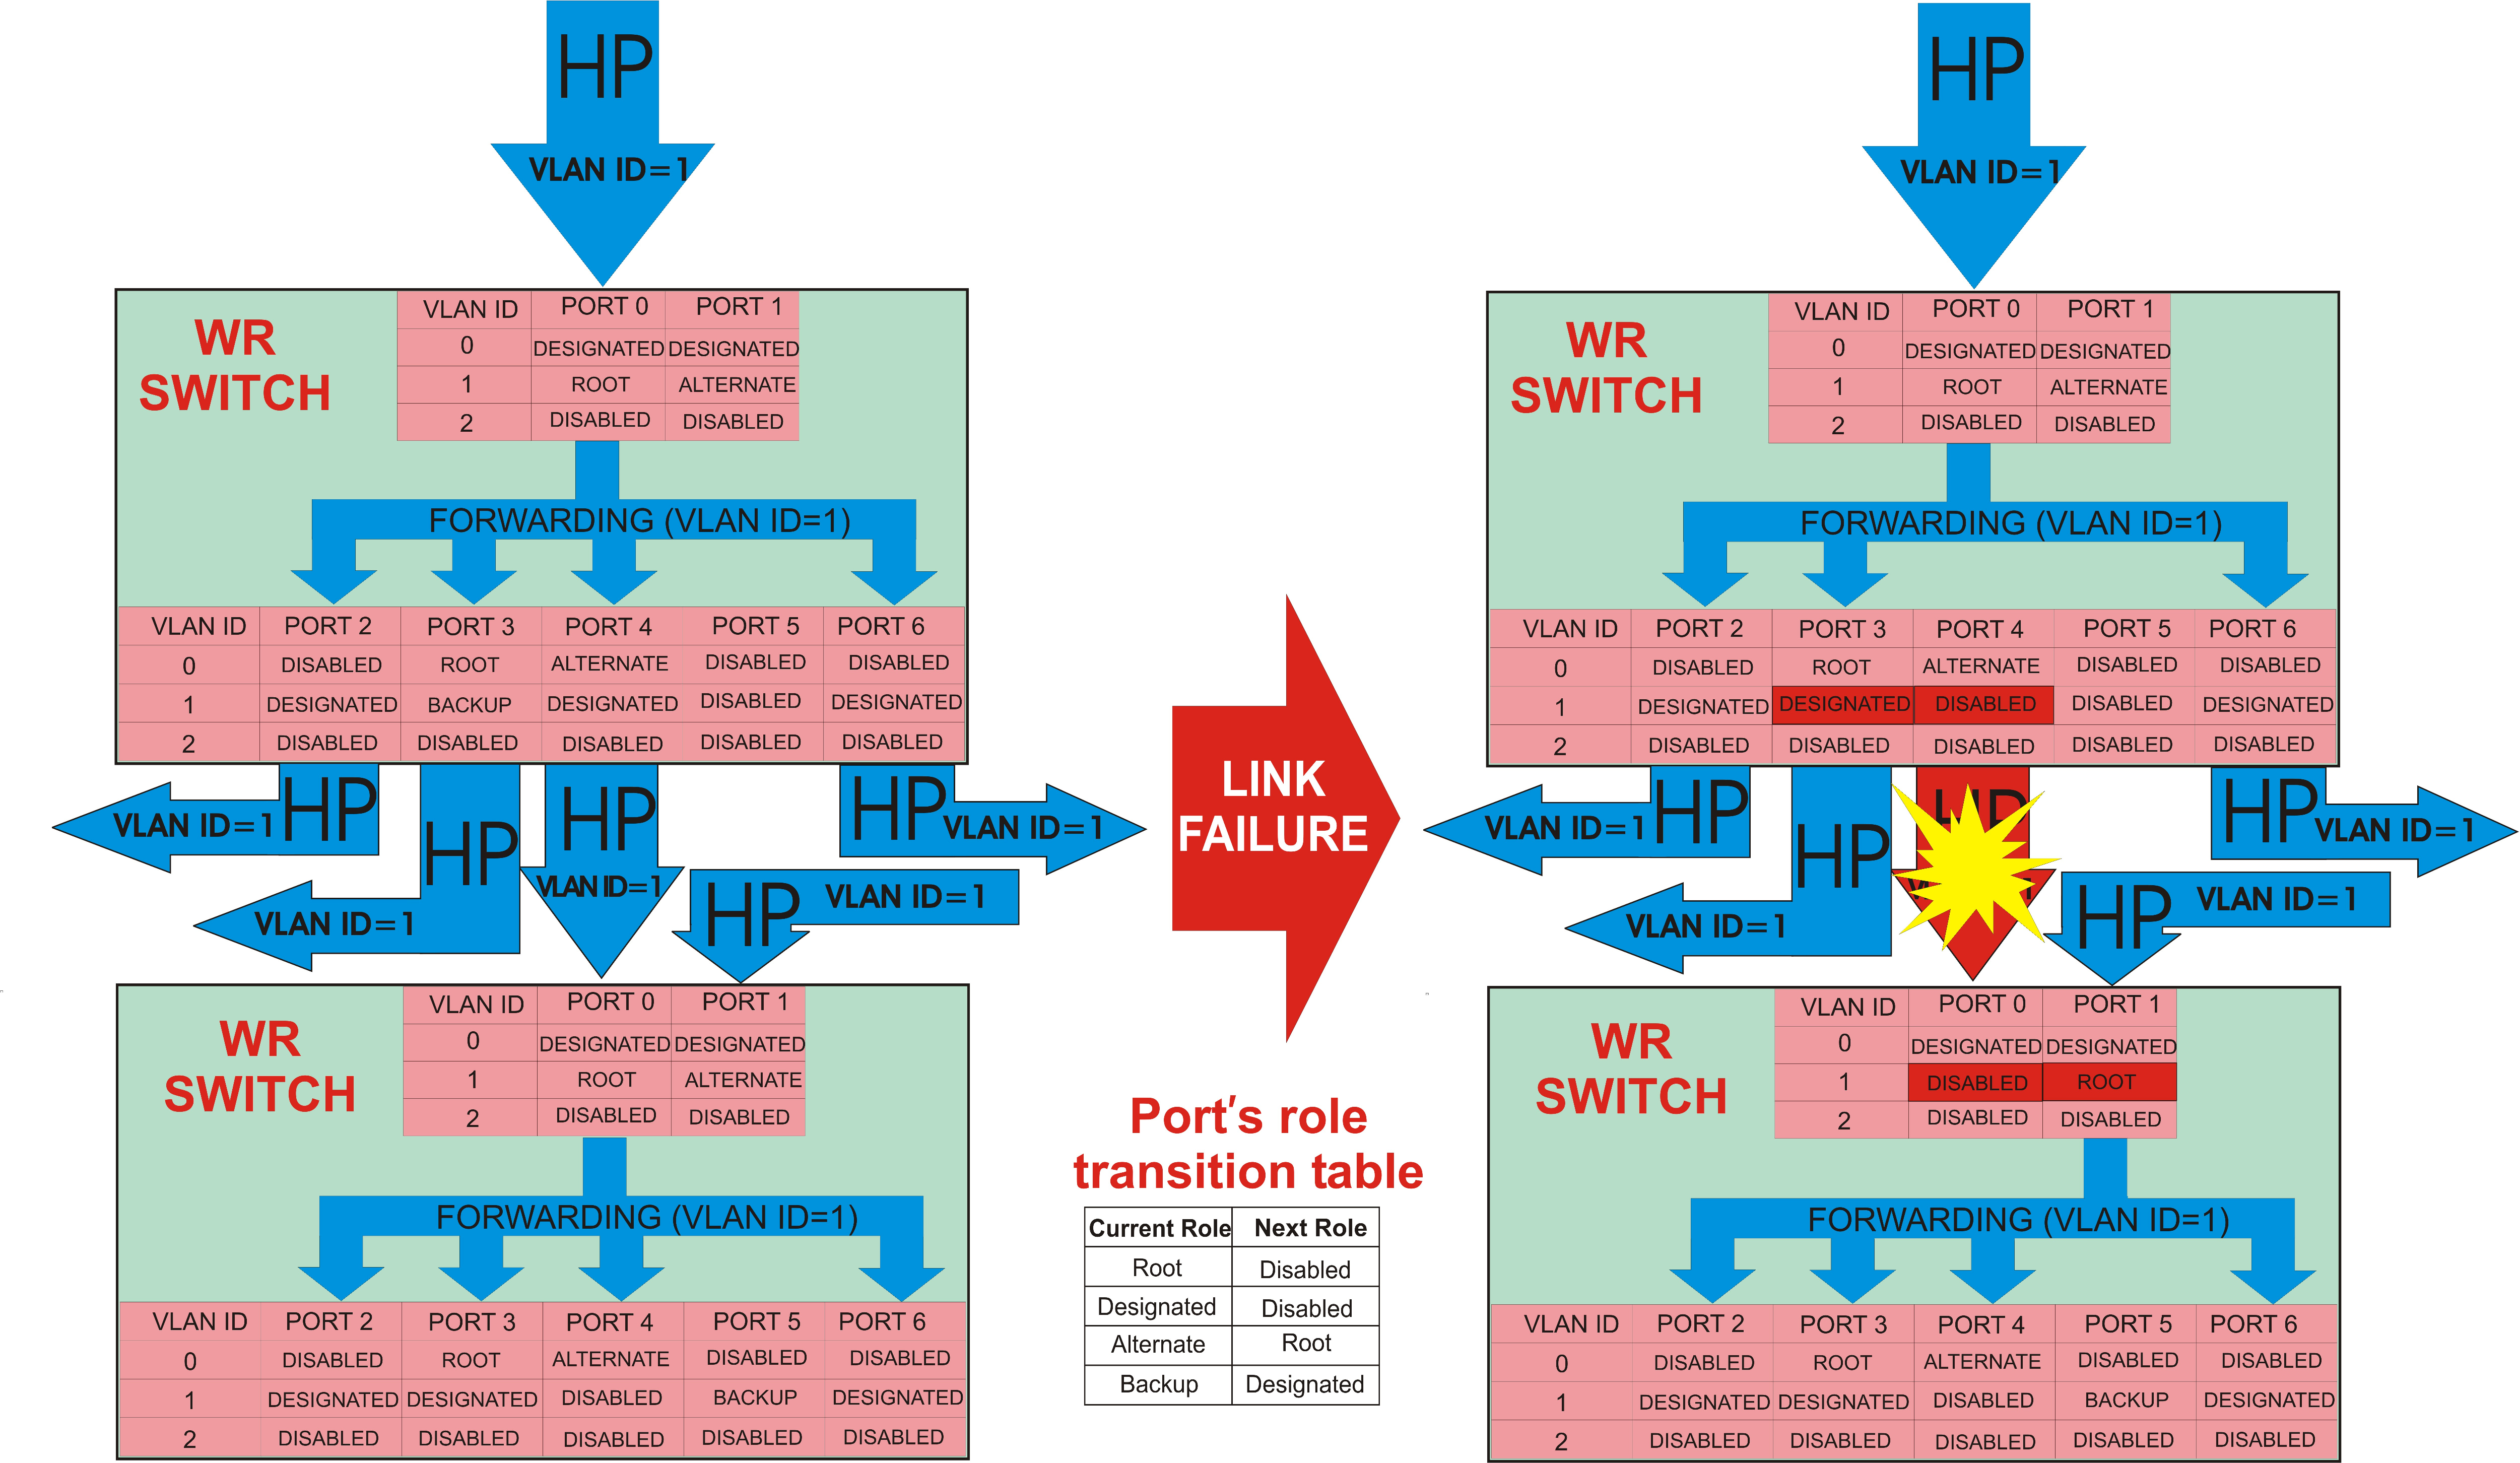
\includegraphics[scale=0.20]{robustness/wrRSTP.ps}
	\captionof{figure}{WR RSTP for HP Traffic}
	\label{fig:wrRSTP}
\end{center}
